\chapter{Analytics Tools used in this research}
This chapter complements the `On Mobile Analytics` chapter. That chapter covers the key elements and concepts, this one describes the analytics tools we used during my research.

\section{Google Play Console incorporating Android Vitals}\label{google_play_console_section}

\subsection{Key Components of Google Play Console}
\subsubsection{Google Play Console UI}

TODO Describe each screen and the contents. Provide a table of the URL mapping and summary of their contents.

Name each graph and provide a screenshot so they can be discussed.

\begin{figure}[htbp]
    \centering
    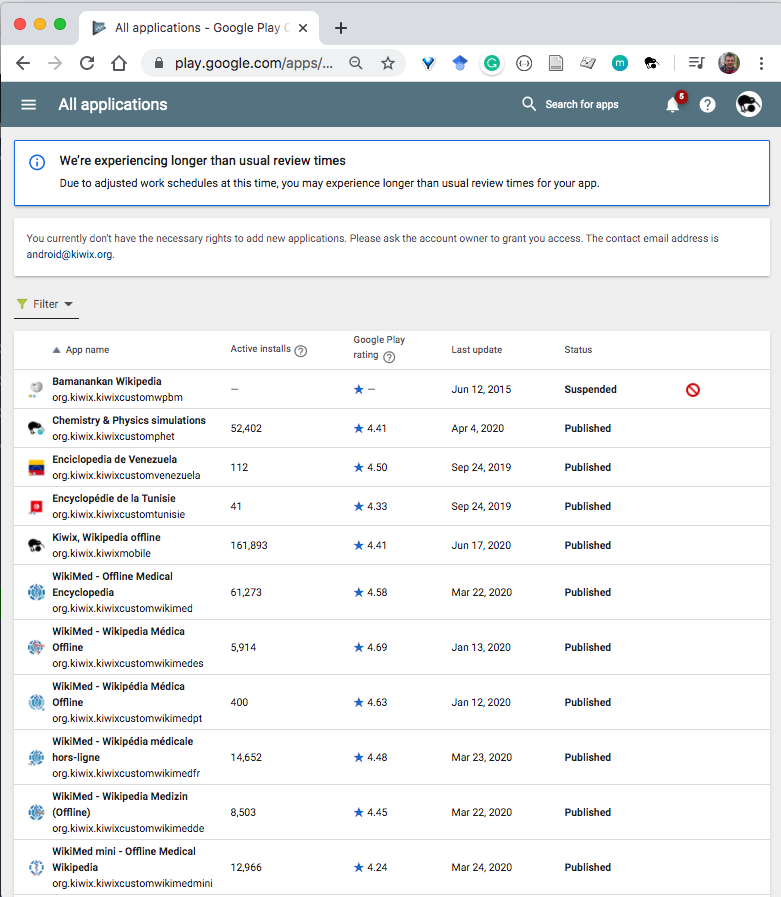
\includegraphics[width=12cm]{images/android-vitals-screenshots/AppListPlace-kiwix-2020-Jun-17.png}
    \caption{Google Play Console: AppListPlace for Kiwix project}
    \label{fig:gpc-applistplace-kiwix}
\end{figure}

\subsection{Pre-launch reports}

~\url{https://stackoverflow.com/questions/48291106/security-warning-in-google-developer-console-pre-launch-reports-security-tab}

\subsection{Android Vitals}
\subsubsection{Android Vitals UI}

\subsubsection{Peer Groups in Android Vitals}\label{android-vitals-peer-groups}
% Google calls them peer groups.
Android Vitals offers developers the option to define a peer group of between 8 and 12 other apps in the Google Play Store. The peer group can be edited up to 3 times per month according to the documentation, and changes seem to take immediate effect in terms of the reporting~\footnote{\url{https://support.google.com/googleplay/android-developer/answer/9324048}}.

The daily crash rate for the peer group can vary which is interesting in terms of observing variations in their overall crash-rate; Figure \ref{fig:pocketcode_peer_crash_rate_18_nov_2019} illustrates the daily change for one of the case studies: the Pocket Code Android app. It is not likely to be easy to determine which of those apps spiked (as the list can only be updated 3 times per month, editing the list and observing the difference has a low likelihood of unmasking the peer, the author will leave designing approaches for future research).

\begin{figure}[ht]
    \centering
    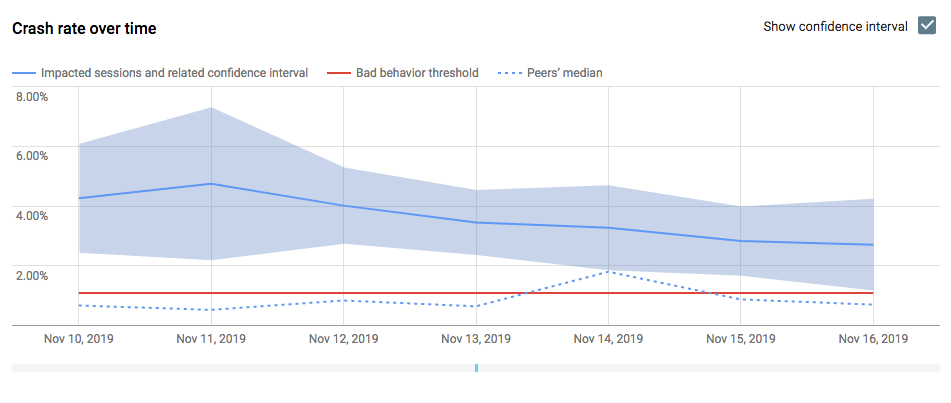
\includegraphics[width=\textwidth]{images/android-vitals-screenshots/peer-crash-rate-catrobat-18-nov-2019.jpg}
    \caption{Pocket Code peer crash-rate as of \nth{18} Nov 2019.}
    \label{fig:pocketcode_peer_crash_rate_18_nov_2019}
\end{figure}{}


\subsection{Monthly Report Files}

Google Play Console generates monthly reports, with the current month's report updated on a daily basis. 

%COULD_DO map screens or graphs to monthly report files.

\subsubsection{Access to the Monthly Report Files}
The reports are only made available for accounts which have 'global' read-only access\emph{`To access bulk reports, your "View app information" permission must be set to "Global."'}~\footnote{\url{https://support.google.com/googleplay/android-developer/answer/6135870\#export}}. Google explain why \emph{``Reports available on Google Cloud Storage use the same access restrictions that control data access on your Play Console. This means account users with access to areas of a Play Console account have access to the corresponding reports in Google Cloud Storage."}~\footnote{\url{https://support.google.com/googleplay/android-developer/answer/2528691}}  


\section{Fabric Crashlytics}

\begin{itemize}
    \item History of Crashlytics:
    \item Crashlytics, one of several products incorporated into Fabric.
    \item Migration of Fabric from Twitter to Google.
    \item Firebase eclipses and supersedes Fabric
\end{itemize}

\url{https://status.firebase.google.com/incident/Crashlytics/20001}

Google retired the Fabric products, including Fabric Crashlytics on \nth{4} May 2020. They provided a range of similar product offerings in Firebase. For Fabric Crashlytics they continue to support the Fabric Client API (presumably so developers did not need to modify their apps to continue collecting crash data) however the reports differ in the Firebase Console, and developers had to explicitly migrate their apps from Fabric to Firebase. The Catrobat development team experienced insurmountable issues trying to migrate all bar one of their Android apps that used Fabric Crashlytics. Seemingly a common flaw also prevents the project team from adding Crashlytics to new apps in their Firebase Account. The workaround the team used was to create a second unrelated account in Firebase and to use that account to configure Crashlytics for apps. %SHOULD-DO discuss the final migration process with Wolfgang and the Android and iOS development teams.

\section{Firebase}
Firebase has come a long way from modest beginnings in 2011~\url{https://techcrunch.com/2012/04/19/firebase-post-launch/} and a change in focus~\url{https://techcrunch.com/2012/05/22/firebase-funding/} through acquisition by Google and further acquisitions~\url{https://www.crunchbase.com/organization/firebase}. Firebase analytics, incorporating Crashlytics, is now by far the most popular analytics library included in Android apps in Google Play. 

\subsection{Firebase Crashlytics}

\subsection{Firebase Analytics}

\section{Microsoft AppCenter}

\section{Summary of Analytics Tools used in this research}
